\documentclass[a4paper, 11pt, fleqn]{book}

\usepackage{graphicx}

% Set equal margins on book style
\setlength{\oddsidemargin}{53pt}
\setlength{\evensidemargin}{53pt}
\setlength{\marginparwidth}{57pt}
\setlength{\footskip}{30pt}

\begin{document}

\title{Objective-C Run-time}
\author{Bc. Kry\u{s}tof V\'{a}\u{s}a}
\date{}
\maketitle 

\chapter{Objective-C}
\section{Foreword}

This thesis will analyze source codes of existing versions of Objective-C run-time, their limitations or requirements for compilation. Result of this work will be a prototype of a modular Objective-C run-time, which will allow easy configuration of the run-time environment both at the compilation and run time. For example, for a single-threaded application, you can turn off the locking of internal structures without affecting stability, yet performance can be improved (with each message sent\footnote{In Objective-C method calls are called messages being sent to objects, just like in Smalltalk.}, a lock can be potentially locked when the method implementation isn't cached and the class hierarchy has to be searched) - this may save quite a few syscalls.

There are three available Objective-C run-time implementations (to my knowledge) - one is provided by Apple and is used in its OS X and iOS systems - there are slight differences between the iOS and OS X versions of the run-time (e.g.\ iOS doesn't support garbage collection and only the new 2.0 run-time is available). Within this thesis, when talking about Apple's implementation of the run-time, the OS X version will be the one talked about. Then there's a run-time provided with GCC and a more experimental one called \'{E}toil\'{e} which is used in a GNUStep-based user environment\footnote{http://www.jot.fm/issues/issue\_2009\_01/article4/index.html}.

Even though I will mention a few words about the garbage collection and ARC\footnote{ARC - automatic reference counting, a feature introduced in Xcode 4.2 (Xcode is Apple's IDE) that uses compiler's static analysis combined with special keywords to automatically insert retain/release calls so that the developer doesn't need to manually manage reference counts on objects.}, not much attention will be paid to them as garbage collection is being deprecated in OS X 10.8 (TODO - ELABORATE IN APPLE SECTION - and has severe dependencies on Mac OS X itself) and ARC is relatively new and uses a lot of compiler-dependent features as well as auto-zeroing weak references, etc.; which is beyond the scope of this work. Instead, the focus will be put on the core functionality of the run-time, analysis of the current implementations and designing the modular run-time itself.
  
\section{Brief history of Objective-C}

In the early 1980s, Brad Cox and Tom Love decided to bring the object-oriented concept to the world of C while maintaining full backward compatibility, strongly inspired by Smalltalk

In 1988, NeXT has licensed Objective-C from Stepstone (the company Cox and Love owned), added Objective-C support to the GCC compiler and decided to use it in its OpenStep and NeXTStep operating systems.

After Apple had acquired NeXT in 1996, Objective-C stayed alive in Rhapsody\footnote{http://en.wikipedia.org/wiki/Rhapsody\_(operating\_system)} and later on in Mac OS X, where it's the preferred programming language to the date.

For this whole time, the Objective-C language stayed almost the same without any significant changes. In 2006, Apple announced Objective-C 2.0 (which was released in Mac OS X 10.5 in 2007), which introduced garbage collection (which has been deprecated in 10.8 in favor of more efficient ARC - automatic reference counting\footnote{http://cocoaheads.tumblr.com/post/17719985728/10-8-objective-c-enhancements}), properties (object variables with automatically generated getters and/or setters with specified memory management), fast enumeration (enumeration over collections in a foreach-style), and some other minor improvements.

Lately, more improvements have been made to Objective-C, most importantly the aforementioned ARC (automatic reference counting). Apple's run-time a hardcoded set of selectors (method names) that handle the memory management, -autorelease, -retain, -release (together called ARR), in particular. ARC automatically inserts these method calls and automatically generates a -dealloc method (which is called when the object is being deallocated) - which requires compiler support, though.

This, however, presents a problem - none of the ARR calls must be called directly in the code - hence you need to convert all of your code to ARC\@. One disadvantage which results in a big advantage - compatibility with all libraries (Apple calls Objective-C libraries frameworks) - this was a big disadvantage of garbage collection: 

You could keep the code as it was as the run-time itself redirected the ARR methods to a no-op function on the fly, however, all linked libraries/frameworks/plugins needed to be recompiled with garbage collection support turned on. This caused two things: mess in the code as if you migrated your code to garbage-collection-enabled environment, it was riddled with ARR calls, however, newly written code typically omitted those calls, making the code inconsistent; and some libraries never got GC support anyway, so you couldn't use them in GC-enabled applications.

In the newest release of OS X 10.8, several new features have been included - default synthesis of getters (in prior versions, you had to declare \verb=@property= in the header file and use \verb=@sythesize= or \verb=@dynamic= in the implementation file - see Syntax of Objective-C), type-safe enums, literals for NSArray, NSDictionary and NSNumber (classes declared in Apple's Foundation framework), etc.

\section{Compilation of Objective-C}

Objective-C is an object-oriented programming language that is a strict superset of C. Any C code can be used within Objective-C source code. Its run-time is written in C as well, some parts in assembly language (mostly performance optimizations) or more recently in C++ (more about that later on). This thesis assumes that you have some brief knowledge of both C and Objective-C, at least syntax-wise.

All Objective-C code can be translated to calls of C run-time functions\footnote{There's a LLVM Clang compiler option -rewrite-objc which will convert all the Objective-C syntax into calls of pure C methods - the run-time methods. When run `clang -rewrite-objc test.m', where test.m contains the Objective-C code, a new test.cpp is created, containing the translated code.} - for example, sending a message to an object isn't anything else than calling a run-time function \verb=objc_msgSend=.

This section will cover compilation of Objective-C code and how it's translated into calling run-time functions.

\subsection{Calling methods}

This is a sample code that sends two messages - each to a different object, though\footnote{As will be explained later on, each class actually consists of two classes - the meta class, which has the +alloc method and the regular class, which has the -init method.}:
\begin{verbatim}SomeClass *myObj = [[SomeClass alloc] init];\end{verbatim}

This will be translated to:
\begin{verbatim}SomeClass *myObj = ((id (*)(id, SEL, ...))(void *)objc_msgSend)
              ((id)((id (*)(id, SEL, ...))(void *)objc_msgSend)
                                  (objc_getClass("SomeClass"),
                                  sel_registerName("alloc")), 
                                  sel_registerName("init"));
\end{verbatim}

Which after removing the casting and adding a little formatting is:

\begin{verbatim}SomeClass *myObj = 
  objc_msgSend(
    objc_msgSend(
      objc_getClass("SomeClass"),  
      sel_registerName("alloc")), 
    sel_registerName("init"));
\end{verbatim}

So it's two nested \verb=objc_msgSend= calls\footnote{There are actually specific functions for methods that return floating point numbers or structures, as these may require special ABI treatment on some architectures.}. \verb=objc_msgSend= is a method that can be said to be the core of Objective-C run-time. It's the most used function of the run-time. Every method call in Objective-C gets translated into this variadic function call, which takes \verb=self= as the first argument (i.e.\ the object that the method is called on, or the message is sent to\footnote{Here can be seen the Smalltalk influence.}), the second argument is a selector (generally the method's name) and can be followed by arguments.

The run-time then looks up the object's class, finds a function that implements this method (so called \verb=IMP=) and calls it. There's a several things to point out:

• method \emph{names} are used. \verb=sel_registerName= is a function that makes sure that for that particular method name only one selector pointer is kept.
• each of the calls goes to a different object. The first call gets to something returned by \verb=objc_getClass= which returns an instance of a meta class (which is an object as well)
• every class consists of two classes - a class pair - one regular of which you create objects and one meta - which typically (unless you manually craft another one) has only one instance: a receiver for class methods (static methods).

If you care to investigate this hierarchy, here's a small example:

\verb=NSObject= class is part of the Foundation framework Apple supplies. Even though its often assumed to be the one and only root class in Objective-C, this is quite incorrect: there can be as many root classes in Objective-C as you wish - \verb=NSProxy= is an example and you can easily create your own.

\begin{verbatim}@interface ClassWithoutSuperclass
@end\end{verbatim}

This will declare a new root class. It has absolutely no functionality - no memory management \verb=retain= and \verb=release=, no \verb=+alloc= method is declared either - you wouldn't be able to even create a new instance of this class without the run-time function \verb=class_createInstance=\footnote{This is basically why it is recommended to inherit everything from NSObject (or any other basic object class) which implements some basic communication with the run-time as well as some basic memory management, etc.}.

Each object is a pointer to a structure. Let's use this simplified class structure (it's more complex in real life):

\begin{verbatim}
typedef struct class_t {
  struct class_t *isa;
  struct class_t *superclass;
} objc_class_t;
\end{verbatim}

Every object is a pointer to a structure like this one. The first field, so-called \verb=isa=, is a pointer to the class structure (to the meta class instance). Second field points to the superclass. It might be confusing at first that it's a class structure, but remember that even the object's class is actually an object - an instance of the meta class\footnote{The root meta class's isa pointer points to the structure itself - i.e. there's a pointer cycle.}.

Assume the following code:
\begin{verbatim}@interface Rootclass
@end
@implementation Rootclass
@end

@interface Subclass : Rootclass
@end
@implementation Subclass
@end 
\end{verbatim}

This declares two classes - \verb=Rootclass= and \verb=Subclass=. The \verb=Rootclass= is a new root class with no superclass. As neither of these classes declares any methods, calling anything on either class would result in a run-time exception, even the usual object creation via \verb=[[Rootclass alloc] init]= isn't available as \verb=Rootclass= doesn't declare the \verb=+alloc= method - it's declared on the \verb=NSObject= class, which is why you can create instances of the ``regular" classes inheriting from \verb=NSObject= this way.

Hence we need to use the run-time \verb=class_createInstance= function to create an instance of the class: 
\begin{verbatim}
id obj = class_createInstance(objc_getClass("Subclass"), 0);
\end{verbatim}

The \verb=objc_getClass= function returns a pointer to the class called \verb=Subclass=, the \verb=objc_getClass= function creates an instance of the \verb=Subclass= class, with \verb=0= extra bytes\footnote{TODO: explain extra bytes.}. Here's a class and meta-class diagram of this situation.

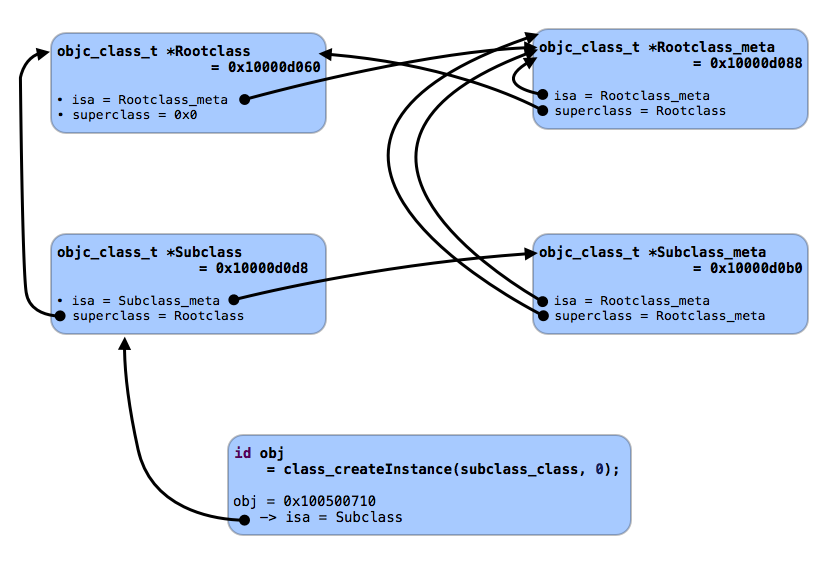
\includegraphics[width=120mm]{metaclass_graph.png}

\subsection{Creating Classes Programmatically}

There is a function called \verb=objc_allocateClassPair= which creates a brand new class and its meta class (together a class pair) on the run. All you need to specify is the superclass, new class name and extra bytes. Using functions such as \verb=class_addMethod=, \verb=class_addIvar=, \verb=class_addProtocol= and \verb=class_addProperty= can be used to add methods, ivars, protocols and properties to a class.

Using these methods, you can easily substitute the Objective-C compiler, creating all classes at the beginning of the application run. 

In reality, declaring a class doesn't cause the compiler to generate function calls, however, instead, the compiler creates static class structures which are later on copied by the linker into the \verb=__OBJC= section of the Mach-O binary (on OS X), which is copied on the launch time to memory and the classes just get registered to the run-time\footnote{Creating the class using the objc\_allocateClassPair function isn't enough in order to create an instance of this class, you need to register the class pair with the run-time as well using objc\_registerClassPair. This is simply to avoid creating an instance of the class before it gets fully initialized, e.g.\ from a different thread.}, which is much faster that dynamically create classes one by one, connecting all methods. We will, however, focus on the run-time methods, ignoring linker dependencies.

\subsection{Translating Methods to Functions}



\begin{verbatim}

@implementation SomeClass
+(void)doSomethingStatic{
  // Nothing to do
}
-(void)secondMethod:(void*)firstArgument withTwoArguments:(int)secondArgument{
    // Do something meaningful, at last!
}
-(void)someMethod:(void*)firstArgument{
    [self secondMethod:firstArgument withTwoArguments:1];
}
@end

\end{verbatim}

\begin{verbatim}
typedef struct objc_object SomeClass;

static void _C_SomeClass_doSomethingStatic(Class self, SEL _cmd) {
  // Nothing to do
}

static void _I_SomeClass_secondMethod_withTwoArguments_
  (SomeClass * self, SEL _cmd, void *firstArgument, 
  int secondArgument) {
  // Do something meaningful, at last!
}

static void _I_SomeClass_someMethod_(SomeClass * self, SEL _cmd, 
  void *firstArgument) {
  ((void (*)(id, SEL, void *, int))(void *)objc_msgSend)((id)self,
     sel_registerName("secondMethod:withTwoArguments:"), 
     (void *)firstArgument, 1);
}

\end{verbatim}


Back to the generated code, though. As you can see, there are two generated functions that correspond to the methods declared by the class \verb=SomeClass=. Their names get slightly obfuscated - \verb=_X_ClassName_method_name_= - where X is either I for instance methods or C for class methods.

First two arguments are always the same - \verb=self= and \verb=_cmd=: \verb=self= points to the object the message is being sent and \verb=_cmd= is the selector (\verb=SEL=). Selector is a structure that consists of just the method's name, so theoretically, it's possible to simply retype \verb=char*= to \verb=SEL= as is being done later on in the method lists. Selectors have generally nothing to do with the actual method implementation.

The first two methods do nothing, hence are uninteresting, but the second one calls (sends a message) its own method \verb=secondMethod:withTwoArguments:=. There's a lot of retyping going on within the call, but generally a function called \verb=objc_msgSend= is called, which lies at the core of all message calls\footnote{There are actually specific functions for methods that return floating point numbers or structures, as these may require special ABI treatment on some architectures.}. The first argument of the function is just passing the \verb=self= variable, for the \verb=_cmd= argument, it uses result of \verb=sel_registerName= - the result is a \verb=SEL= and this method makes sure that for selectors with the same name, the same pointer is returned - i.e. two objects with a method with the same name get the same \verb=SEL= pointer. The third argument is quite self-explanatory.


\chapter{Apple's Implementation}
\section{Limitations}
// TODO
- Bridging, 16B objects minimum.

\end{document}
      